\chapter{Thesis Background}
\label{sec:backgroundthesis}

This chapter is about the background of the thesis, in order to understand better further chapters and as a help and reference to reproduce the results of this thesis in the future. 

\section{PYNQ-Z2 Development Board}
The \textit{PYNQ-Z2} is a development board designed for the Xilinx University Program. It is equipped with a Xilinx ZYNQ 7020 SoC (XC7Z020-1CLG400C), 512 MB of DDR3 RAM and 16 MB of QSPI Flash Storage. The board provides a clock reference thanks to a crystal oscillator with a frequency of 50 MHz. The reference clock is used by the PS and can be provided to the PL too. 

\begin{figure}[H]
\centering
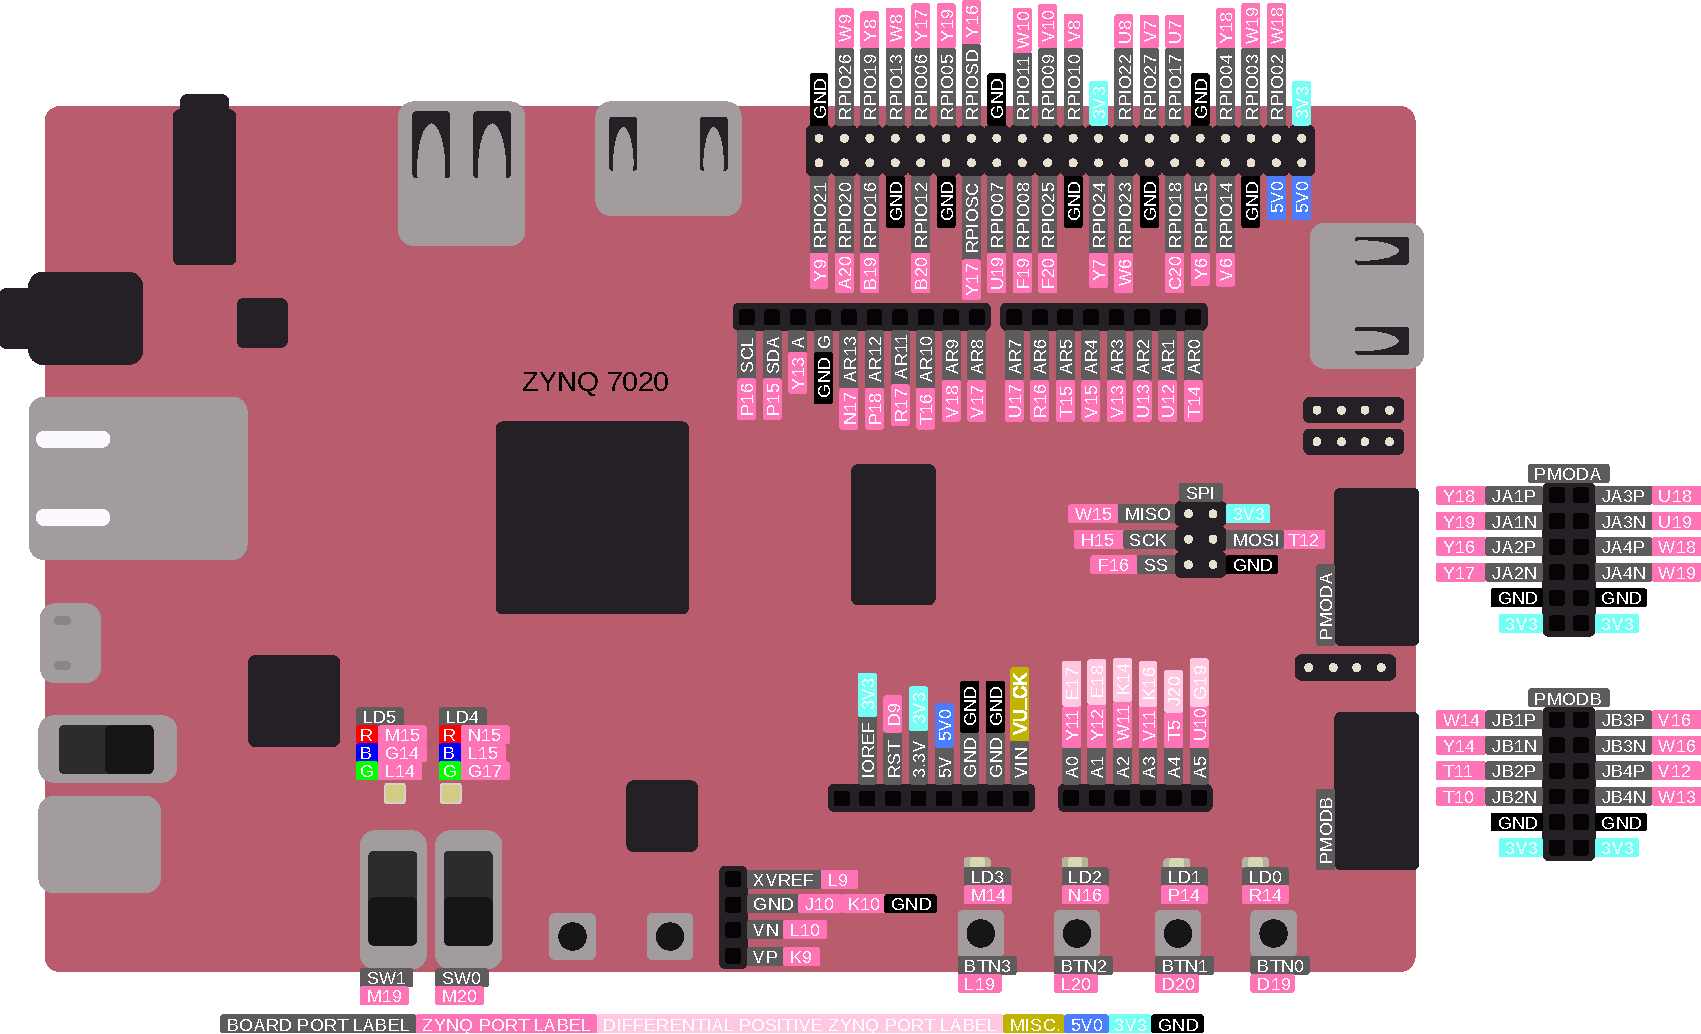
\includegraphics[width=0.7\linewidth]{images/chapter3/PINOUT.pdf}
\caption{Schematic of the PYNQ-Z2 Development Board}
\label{fig:pynqz2}
\end{figure}

The SoC is made of two subparts: a Processing System (PS) and a Programmable Logic (PL). The PS is the main part of the SoC, containing two 650 MHz ARM Cortex-A9 processor, 512 KB L2 Cache, 256 KB On-Chip Memory and other modules like FPUs, Flash Controller, DRAM Controller, GPIOs and so on.

\begin{figure}[H]
\centering
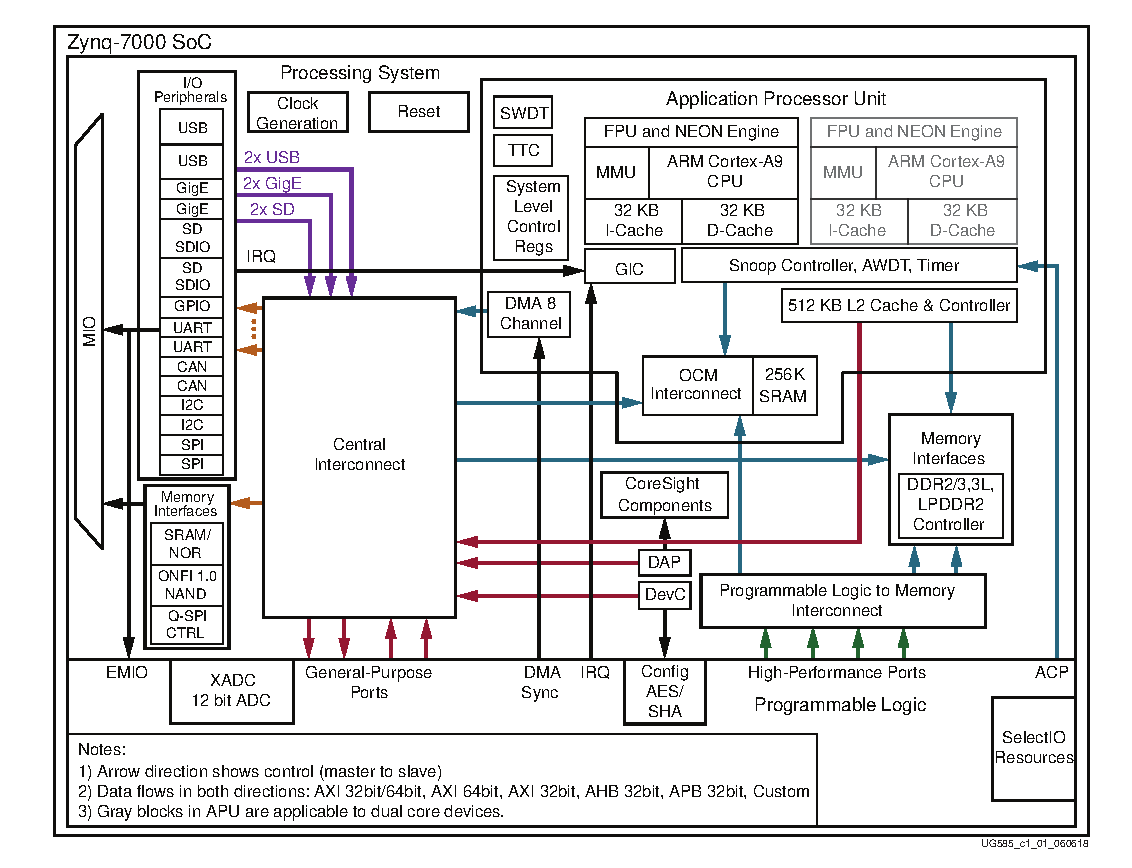
\includegraphics[width=1.0\linewidth]{images/chapter3/zynq.pdf}
\caption{Schematic of ZYNQ 7020 SoC}
\label{fig:zynq7020}
\end{figure}

A schematic is shown in Figure \ref{fig:zynq7020}. The second part is the PL, which consists in a FPGA with the following characteristics:

\begin{itemize}
    \item 13,300 logic slices, each with four 6-input LUTs and 8 flipflops
    \item 630 KB block RAM (BRAM)
    \item 220 DSP slices
    \item On-chip Xilinx analog-to-digital converter (XADC)
\end{itemize}

The PL can access the Processing System's memory space, as shown in Table \ref{tab:zynq_memory_map}, through a High Performance and/or General Purpose AXI Ports. This enables the usage, for example, of the DDR3 RAM and of the On-Chip memory (OCM) from the PL. The board can be programmed through a JTAG interface, which allows to upload a firmware to be executed from the PS or to program the PL via a bitstream. Moreover, it provides a virtual UART interface that can be used as input/output both for the PS and the PL.\bigskip

\begin{table}[ht]
\centering
\begin{tabular}{ |p{3cm}||p{3cm}||p{5cm}|  }
    \hline
    \multicolumn{3}{|c|}{Memory Mapping} \\
    \hline
    Address Start&Address End&Device \\
    \hline
    \texttt{0x00000000}&\texttt{0x3FFFFFFF}&DDR \& OCM\\
    \texttt{0x40000000}&\texttt{0xBFFFFFFF}&PL  \\
    \texttt{0xC0000000}&\texttt{0xDFFFFFFF}&Reserved\\
    \texttt{0xE0000000}&\texttt{0xE02FFFFF}&Memory mapped devices\\
    \texttt{0xE0300000}&\texttt{0xE0FFFFFF}&Reserved\\
    \texttt{0xE1000000}&\texttt{0xE3FFFFFF}&NAND, NOR\\
    \texttt{0xE4000000}&\texttt{0xE5FFFFFF}&SRAM\\
    \texttt{0xE6000000}&\texttt{0xF7FFFFFF}&Reserved\\
    \texttt{0xF8000000}&\texttt{0xF8FFFFFF}&AMBA APB Peripherals\\
    \texttt{0xF9000000}&\texttt{0xFBFFFFFF}&Reserved\\
    \texttt{0xFC000000}&\texttt{0xFDFFFFFF}&Linear QSPI - XIP\\
    \texttt{0xFE000000}&\texttt{0xFFEFFFFF}&Reserved\\
    \texttt{0xFFF00000}&\texttt{0xFFFFFFFF}&OCM \\
    \hline
\end{tabular}
\caption{ZYNQ 7020 SoC Memory Map}
\label{tab:zynq_memory_map}
\end{table}

% \begin{bytefield}{24}
%     \memsection{0xffff\_ffff}{0xfff0\_0000}{3}{PL}\\
%     \memsection{0xffef\_ffff}{0xfe00\_0000}{3}{PL}\\
%     \memsection{0xfdff\_ffff}{0xfc00\_0000}{3}{PL}\\
%     \memsection{0xfbff\_ffff}{0xf900\_0000}{3}{PL}\\
%     \memsection{0xf8ff\_ffff}{0xf800\_0000}{3}{PL}\\
%     \memsection{0xf7ff\_ffff}{0xe600\_0000}{3}{PL}\\
%     \memsection{0xe5ff\_ffff}{0xe400\_0000}{3}{PL}\\
%     \memsection{0xe3ff\_ffff}{0xe100\_0000}{3}{PL}\\
%     \memsection{0xe0ff\_ffff}{0xe030\_0000}{3}{PL}\\
%     \memsection{0xe02f\_ffff}{0xe000\_0000}{3}{PL}\\
%     \memsection{0xdfff\_ffff}{0xc000\_0000}{3}{PL}\\
%     \memsection{0xbfff\_ffff}{0x4000\_0000}{3}{PL}\\
%     \memsection{0x3fff\_ffff}{0x0000\_0000}{3}{OCM/DDR}
% \end{bytefield}


%%%%%%%%%%%%%%%%%%%%%%%%%%%%%%%%%%%%%%%%%%%%%%%%%%%%%%%%%%%%%%%%%%%%%%%%%
%%%%%%%%%%%%%%%%%%%%%%%%%%%%%%%%%%%%%%%%%%%%%%%%%%%%%%%%%%%%%%%%%%%%%%%%%
%%%%%%%%%%%%%%%%%%%%%%%%%%%%%%%%%%%%%%%%%%%%%%%%%%%%%%%%%%%%%%%%%%%%%%%%%
%%%%%%%%%%%%%%%%%%%%%%%%%%%%%%%%%%%%%%%%%%%%%%%%%%%%%%%%%%%%%%%%%%%%%%%%%
%%%%%%%%%%%%%%%%%%%%%%%%%%%%%%%%%%%%%%%%%%%%%%%%%%%%%%%%%%%%%%%%%%%%%%%%%
%%%%%%%%%%%%%%%%%%%%%%%%%%%%%%%%%%%%%%%%%%%%%%%%%%%%%%%%%%%%%%%%%%%%%%%%%
%%%%%%%%%%%%%%%%%%%%%%%%%%%%%%%%%%%%%%%%%%%%%%%%%%%%%%%%%%%%%%%%%%%%%%%%%
%%%%%%%%%%%%%%%%%%%%%%%%%%%%%%%%%%%%%%%%%%%%%%%%%%%%%%%%%%%%%%%%%%%%%%%%%
%%%%%%%%%%%%%%%%%%%%%%%%%%%%%%%%%%%%%%%%%%%%%%%%%%%%%%%%%%%%%%%%%%%%%%%%%
%%%%%%%%%%%%%%%%%%%%%%%%%%%%%%%%%%%%%%%%%%%%%%%%%%%%%%%%%%%%%%%%%%%%%%%%%
%%%%%%%%%%%%%%%%%%%%%%%%%%%%%%%%%%%%%%%%%%%%%%%%%%%%%%%%%%%%%%%%%%%%%%%%%
% \subsection{Configuration Ports}
%%%%%%%%%%%%%%%%%%%%%%%%%%%%%%%%%%%%%%%%%%%%%%%%%%%%%%%%%%%%%%%%%%%%%%%%%
%%%%%%%%%%%%%%%%%%%%%%%%%%%%%%%%%%%%%%%%%%%%%%%%%%%%%%%%%%%%%%%%%%%%%%%%%
%%%%%%%%%%%%%%%%%%%%%%%%%%%%%%%%%%%%%%%%%%%%%%%%%%%%%%%%%%%%%%%%%%%%%%%%%
%%%%%%%%%%%%%%%%%%%%%%%%%%%%%%%%%%%%%%%%%%%%%%%%%%%%%%%%%%%%%%%%%%%%%%%%%
%%%%%%%%%%%%%%%%%%%%%%%%%%%%%%%%%%%%%%%%%%%%%%%%%%%%%%%%%%%%%%%%%%%%%%%%%
%%%%%%%%%%%%%%%%%%%%%%%%%%%%%%%%%%%%%%%%%%%%%%%%%%%%%%%%%%%%%%%%%%%%%%%%%
%%%%%%%%%%%%%%%%%%%%%%%%%%%%%%%%%%%%%%%%%%%%%%%%%%%%%%%%%%%%%%%%%%%%%%%%%
%%%%%%%%%%%%%%%%%%%%%%%%%%%%%%%%%%%%%%%%%%%%%%%%%%%%%%%%%%%%%%%%%%%%%%%%%
%%%%%%%%%%%%%%%%%%%%%%%%%%%%%%%%%%%%%%%%%%%%%%%%%%%%%%%%%%%%%%%%%%%%%%%%%
%%%%%%%%%%%%%%%%%%%%%%%%%%%%%%%%%%%%%%%%%%%%%%%%%%%%%%%%%%%%%%%%%%%%%%%%%
%%%%%%%%%%%%%%%%%%%%%%%%%%%%%%%%%%%%%%%%%%%%%%%%%%%%%%%%%%%%%%%%%%%%%%%%%

\section{Xilinx's Microblaze soft-core}

The Microblaze is a soft-core (or soft-microprocessor) designed for Xilinx's FPGAs. Introduced in 2002, it is based on a RISC architecture, with an ISA (Instruction Set Architecture) similar to the DLX architecture. It is a pipelined processor and, with few exceptions, the MicroBlaze can issue a new instruction every cycle, maintaining single-cycle throughput under most circumstances.\bigskip

The Microblaze has an interface to the AXI Interconnect, used to connect to other peripherals and memories. It has a dedicated bus, LMB Bus, for access to local-memory (FPGA's BRAMs): this can be used both for Instruction (ILMB) and Data (DLMB) storage.

\begin{figure}[H]
\centering
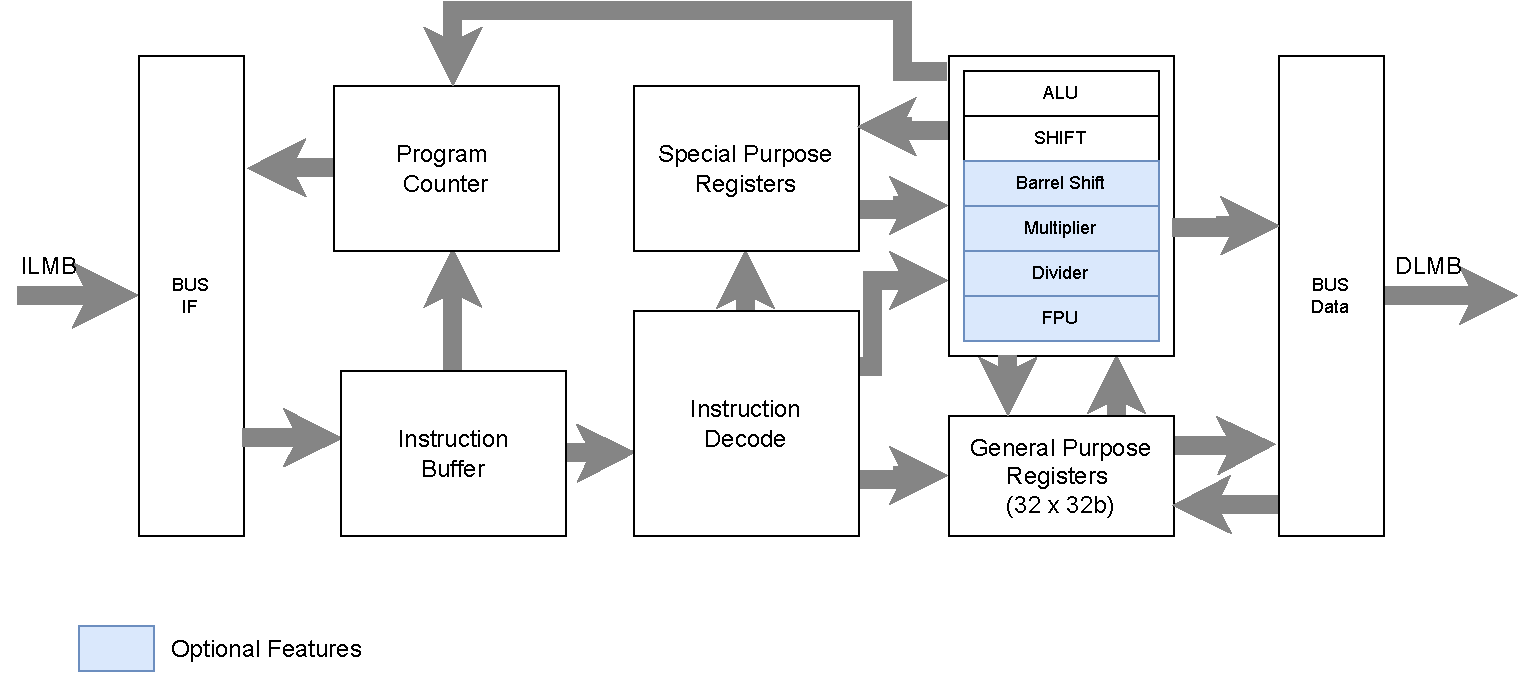
\includegraphics[width=0.8\linewidth]{images/chapter3/ublaze_arch.pdf}
\caption{\cite{anemaet2003microprocessor}Overview of a Microblaze SoftCore}
\label{fig:ublaze}
\end{figure}

A general overview of the Microblaze architecture is shown in Figure \ref{fig:ublaze}. Because it is meant for FPGAs, and FPGAs are flexible by construction, a Microblaze instance can be personalized in many ways to fit the user's needs. Example of configurations are the cache size (or the cache can be enabled or disabled at all), pipeline depth (3-stage, 5-stage, or 8-stage) and bus-interfaces. There are some presets, like the area-optimized one which uses a 3-stage pipeline and sacrifices clock frequency for reduced logic area. The performance-optimized preset expands the execution pipeline to 5 stages. One of the most important configuration is related to the supported ISA: key processor instructions which are rarely used but more expensive to implement in hardware can be selectively added/removed (e.g. multiply, divide, and floating point operations).

\section{Xilinx FPGA Standard Design Flow}

Xilinx offers a software suite for Xilinx's FPGAs. The provided software suite is \textit{Vivado Design Suite}, and this thesis has been developed using version 2021.1. The suite supports designers in all the steps of the design process, from the initial HDL design to the final FPGA bistream generation. At each stage of the design flow, the design can perform analysis and verification, by performing logical simulations of the design, estimation of power consumption, constraints definition, I/O and clock planning, design rule checks (DRC) and modification of implementation results.\bigskip

Together with the HDL description, Vivado offers an IP catalog. IP stands for Intellectual Property, and each IP is an already developed and tested design ready to be integrated into the user's own design. An example of IP offered by default is the Microblaze IP, that containts the Microblaze core. The Vivado's Catalog is a comprehensive list of all the IP offered by different repositories: Xilinx's IP, IP obtained from third parties, and end-user designs targeted for reuse as IP into a single environment. \bigskip

One of the key features of the Vivado Design Suite is the choiche given to the user to perform the design flow by means of the Graphical User Interface (GUI) or by TCL commands. The GUI, known as as \textit{Vivado Integrated Design Environment} (IDE), allows the user to follow the evolution of the design visually from the HDL and IP instantiation up to its implementation on physical resources. The TCL commands allow the user to control the design flow by means of scripts. The interesting thing is that each action performed by the user in the GUI corresponds to an exact TCL command that can be seen from the TCL Console available in the IDE. This allow the user to understand what is the TCL command for that specific action and to script the design flow easily. 

\subsection{Steps towards the Bitstream Generation}

In the end, a design can be a combination of IPs and manual HDL code or it can be a full IP-centric design, where the user instantiate the IPs he/she wants to use and interconnect them (usually via AXI Interface but also via other interfaces or custom interfaces, it depends on the IP). For the IP-centric design flow, Vivado offers the \textit{Block Design} tool, which allows the user to visually instantiate e move and connect IPs visually, where each IP corresponds to a block, and to connect them by drawing connections similar to a schematic or using connection automation features provided with a set of DRCs (to ensure proper IP configuration and connectivity), as shown in Figure \ref{fig:block_design_example}. \bigskip

% include image
\begin{figure}[H]
\centering
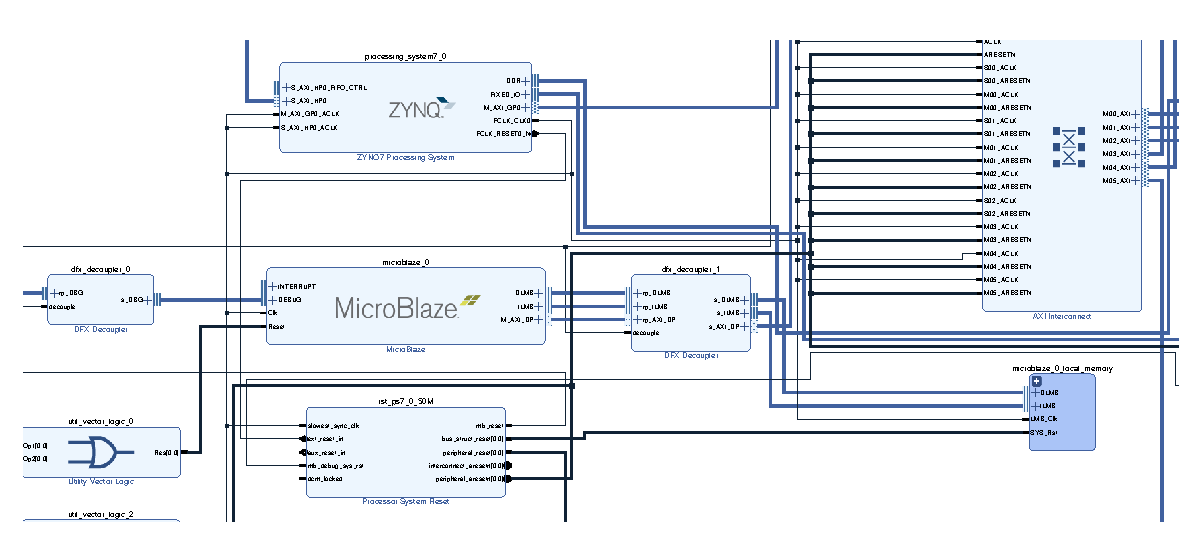
\includegraphics[width=0.8\linewidth]{images/chapter3/design_example-cropped.pdf}
\caption{Example of Block Design}
\label{fig:block_design_example}
\end{figure}

\subsection{Fundamentals of the Xilinx's Bitstream structure}
\subsection{Software Development}
% talk about Vitis and xsct
\section{Fault Injection Tool}